\documentclass[]{article}
\usepackage{graphicx}
\usepackage[table]{xcolor}

%plots path
\graphicspath{ {plots/} }


\title{Impacts of sagebrush vegetation in a desert climate on the atmospheric boundary layer}
\author{Byron Eng, Matthew Moody, and Travis Morrison}

\begin{document}

\maketitle

\begin{abstract}
XXX
\end{abstract}

\section{Introduction}

\section{Results}
Data was provided from the Sagebrush and Playa sites for October 18-19th. Both sites harvested data from meteorological towers equipped with fast response sonic anemometers at multiple heights (18.8 m, 10.15 m, 5.87 m, 2.04 m, and 0.55 m for Sagebrush and 25.5 m,19.4 m, 10.4 m, 5.3 m, 2.02 m, 0.61m for Playa). The variables of interest measured were the three components of velocity (captured at 20 Hz), temperature, relative humidity (captured at 1 Hz). As a post-processing step the analysis,  velocity data components were rotated based on 30-minute block averages, with $u$ denoting the mean wind direction, $v$ as the velocity horizontally perpendicular to the mean flow, $u$, and $w$ as the vertical velocity. Fluctuations from the mean were also calculated from a 30-minute block average. 

% Byron talks about part 1)

%Part 2 and 3~ Travis
To better understand the impacts of vegetation on boundary layer flow, examination of a highly convective time, 1500-1530 MST (2100-2130 UCT), was further analyzed. Characteristics of this period include a mean wind speed and direction of.... . 
The Probability Distribution Function (PDF) for this time period was calculated for each velocity component and temperature at all heights (Figure \ref{fig:pdf}). The largest contrast between the two sites exist between the mean wind velocity component and the temperature. Beginning with $u$ at the sagebrush site the velocity distribution's mean value shifts towards larger values with height, while at the Playa a more uniformed mean velocity is maintained with height. Additionally, differences between the temperature PDF's between the two sites can be observed. At the Sagebrush site, the lower two heights (0.55 and 2.04 m) report much larger mean temperature values ($\sim$19.5$^\circ$ C) than the other heights ($\sim$19.5$^\circ$ C) , while at the Playa site, the temperature varies less with height ($\sim$ 15-16.5 $^\circ$ C). Note at the Sagebrush site the temperature PDF at 0.55 m shows the largest variance. These features can potentially be attributed to the vegetation. Due to the low surface vegetation at the Sagebrush site, increased drag reduces the near surface velocity and increases energy storage (higher surface temperature).  

NEED SOURCES

Examination of this idea can be further seen in Table \ref{tab:kurt_sage} and Table \ref{tab:kurt_playa}, where the kurtosis and skewness is presented with height and variable. The red and blue color boxes correlate to the near surface $u$ velocity. At the Sagebrush the skewness nears 0 at the surface, increasing with height and a kurtosis less than 3. While at the Playa, there is a positive skew near the surface, which decreases with height with a decreasing kurtosis. 

Figure \ref{fig:cdf} presents the Cumulative Distribution Function (CDF). Focusing on the third row (CDF $w$) one can now see of the increased distribution of vertical velocities with height at both heights. This is due to the convective nature of the period of interest. Figure \ref{fig:autocorr} presents the autocorrelation function for the velocity components and the temperature at both sites. The autocorrelation was computed for the 30 minutes of interest, 15 minutes is presented. $u$, $v$, and $T$ show fairly linearly decays in time, while $w$ decays rapidly to 0. Interesting features in Figure \ref{fig:autocorr} are seen in the autocorrelation of $u$ at the Sagebrush and Playa. At the Sagebrush we observe a more rapid decay of correlation at the lower heights, while at the Playa, all heights remain share the same correlation with time. 

It appears the increased mixing at the surface of the Sagebrush creates a more equally well distributed velocity. 



%plot PDFs
\begin{figure}
	\centering
	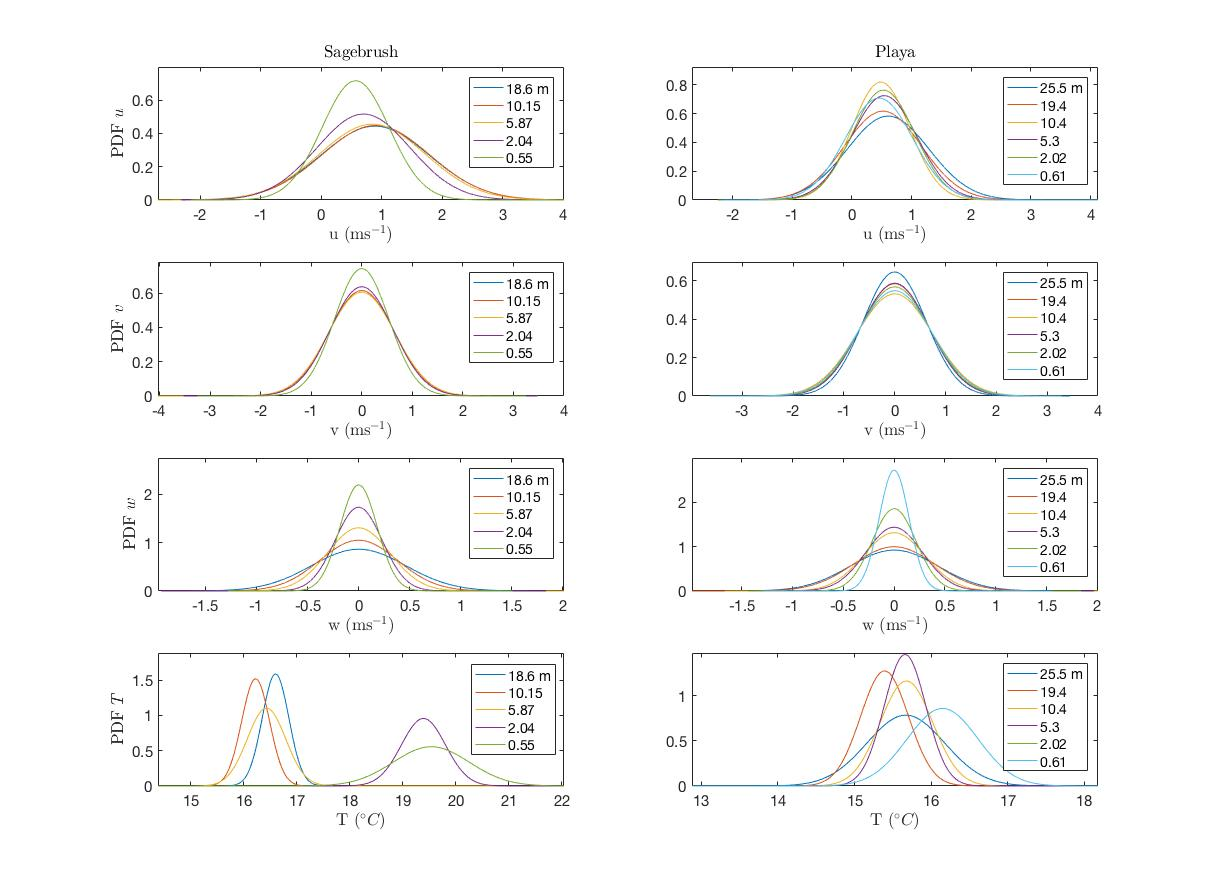
\includegraphics[width=\textwidth]{pdf}
	\caption{Collection of probability distributions from the Sagebrush (\textbf{left}) and the Playa (\textbf{right} sites). From top to bottom PDF $u$, PDF $v$,  PDF $w$ and PDF $T$ . }
	\label{fig:pdf}
\end{figure}

%Create table of Skewness and Kurtosis
\begin{table}
\begin{tabular}{ |p{1cm}|p{2cm}|p{1cm}|p{1cm}|p{1cm}| p{1.5cm}|}

		\hline
		\multicolumn{6}{|c|}{Sagebrush} \\
		\hline\hline
		z (m) & Statistic & u &  v & w & T\\
		\hline
		18.6 & Kurtosis & 2.3731 & 3.1820 & 3.6346&  1.6588\\
		&Skewness & 0.3067 & 0.2446 & 0.8532 & -0.3490\\
		\hline
		10.15 & Kurtosis & 2.4933 & 3.4515 & 2.8027 &1.8469 \\
		&Skewness & 0.1651 & 0.1227 & 0.3879& -0.5126\\
        \hline
       	5.87 & Kurtosis & 2.6679 & 3.2820 & 3.8053 &2.0491 \\
       	&Skewness & 0.2694 & 0.1717 & 0.5359 & -0.6396\\
       	\hline
   		2.04 & Kurtosis & \cellcolor{red!25} 2.6868 & 3.6466  & 3.3045 & 2.0662  \\
   		&Skewness & \cellcolor{blue!25} 0.1876 & 0.3174 & 0.4101& -0.4458\\
   		\hline
		0.55 & Kurtosis & \cellcolor{red!25} 2.6739 & 3.1869 & 3.8168  & 2.4663\\
		&Skewness &\cellcolor{blue!25} 0.0655 & 0.3693 & 0.3859&0.7037\\
		\hline
		
\end{tabular}
\label{tab:kurt_sage}
\caption{Skewness and kurtosis values for the Sagebrush site on October 19th from 1500-1530 MST. }
\end{table}
\begin{table}
\begin{tabular}{ |p{1cm}|p{1.5cm}|p{1cm}|p{1.25cm}|p{1cm}| p{1.25cm}|}
	\hline
	\multicolumn{6}{|c|}{Playa} \\
	\hline\hline
	z (m) & Statistic & u &  v & w & T\\
	\hline
	25.5 & Kurtosis & 2.1075 & 2.5910 & 3.5269 &  2.2656\\
	&Skewness & 0.1212 & -0.2004 & 0.7672 & 0.5295\\
	\hline
	19.4 & Kurtosis & 2.2519 & 2.8332 & 3.4123 &1.6080 \\
	&Skewness & 0.2287 & -0.2862 & 0.7324 & 0.1421\\
	\hline
	10.4 & Kurtosis & 2.8320 & 1.9469 & 3.0079 &4.6 \\
	&Skewness & 0.3884 & 0.1464 & 0.3786 &1.2276\\
	\hline
	5.3 & Kurtosis & 2.9033 & 2.1528  & 3.1285 & 3.2123  \\
	&Skewness & 0.1862 & 0.1298 & 0.4560 & 0.9190\\
	\hline
	2.02 & Kurtosis &\cellcolor{red!25} 3.0038 & 2.0993 & 3.2620  & 2.3460\\
	&Skewness & \cellcolor{blue!25} 0.3980 & -0.0969 & 0.4160 & 0.6531\\
	\hline
	0.61 & Kurtosis & \cellcolor{red!25} 3.1414 & 1.9599 & 3.3634  & 2.3473\\
	&Skewness & \cellcolor{blue!25} 0.5253 & -0.1403 & 0.2770 &0.6531\\
	\hline
\end{tabular}
\label{tab:kurt_playa}
\caption{Skewness and kurtosis values for the Playa site on October 19th from 1500-1530 MST. }
\end{table}
%plot CDFs
\begin{figure}
\centering
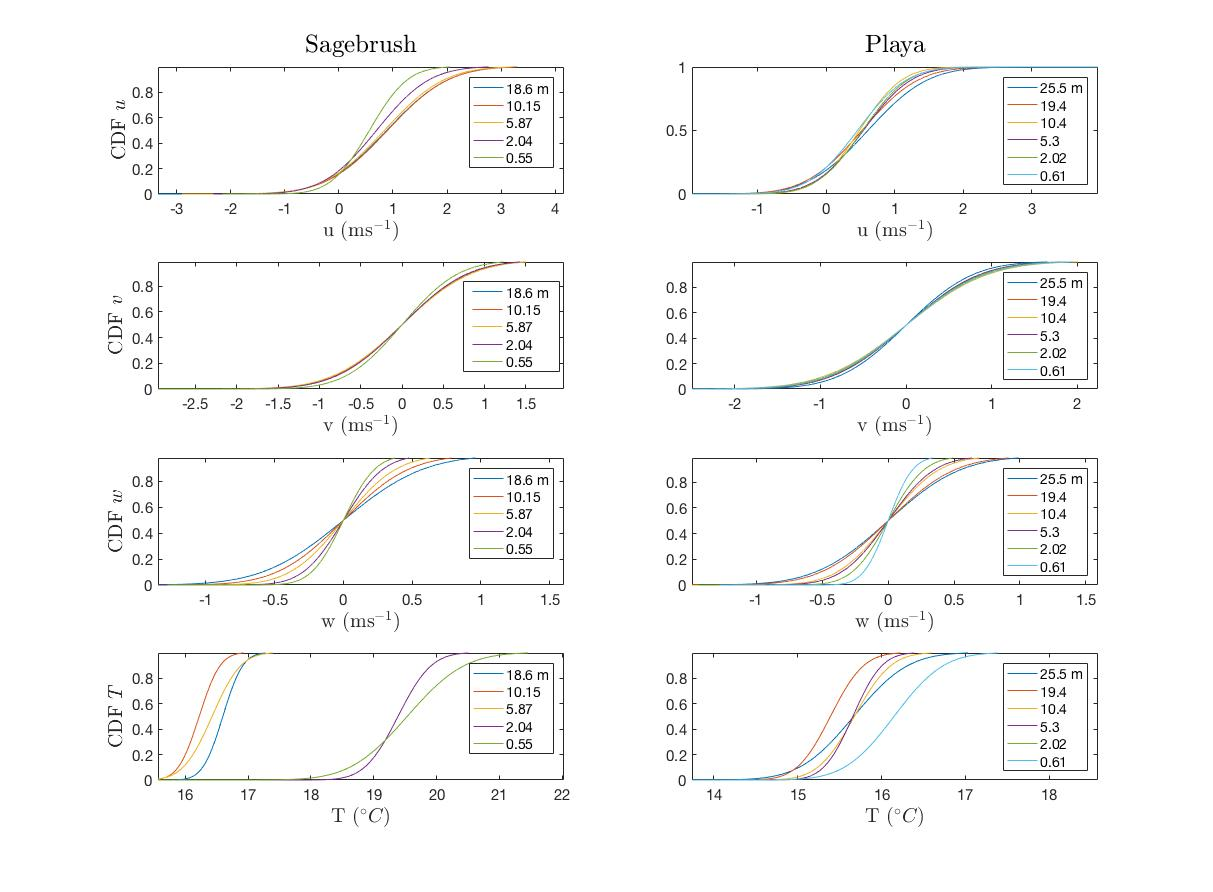
\includegraphics[width=\textwidth]{cdf}
\caption{}
\label{fig:cdf}
\end{figure}

%plot Autocorr
\begin{figure}
	\centering
	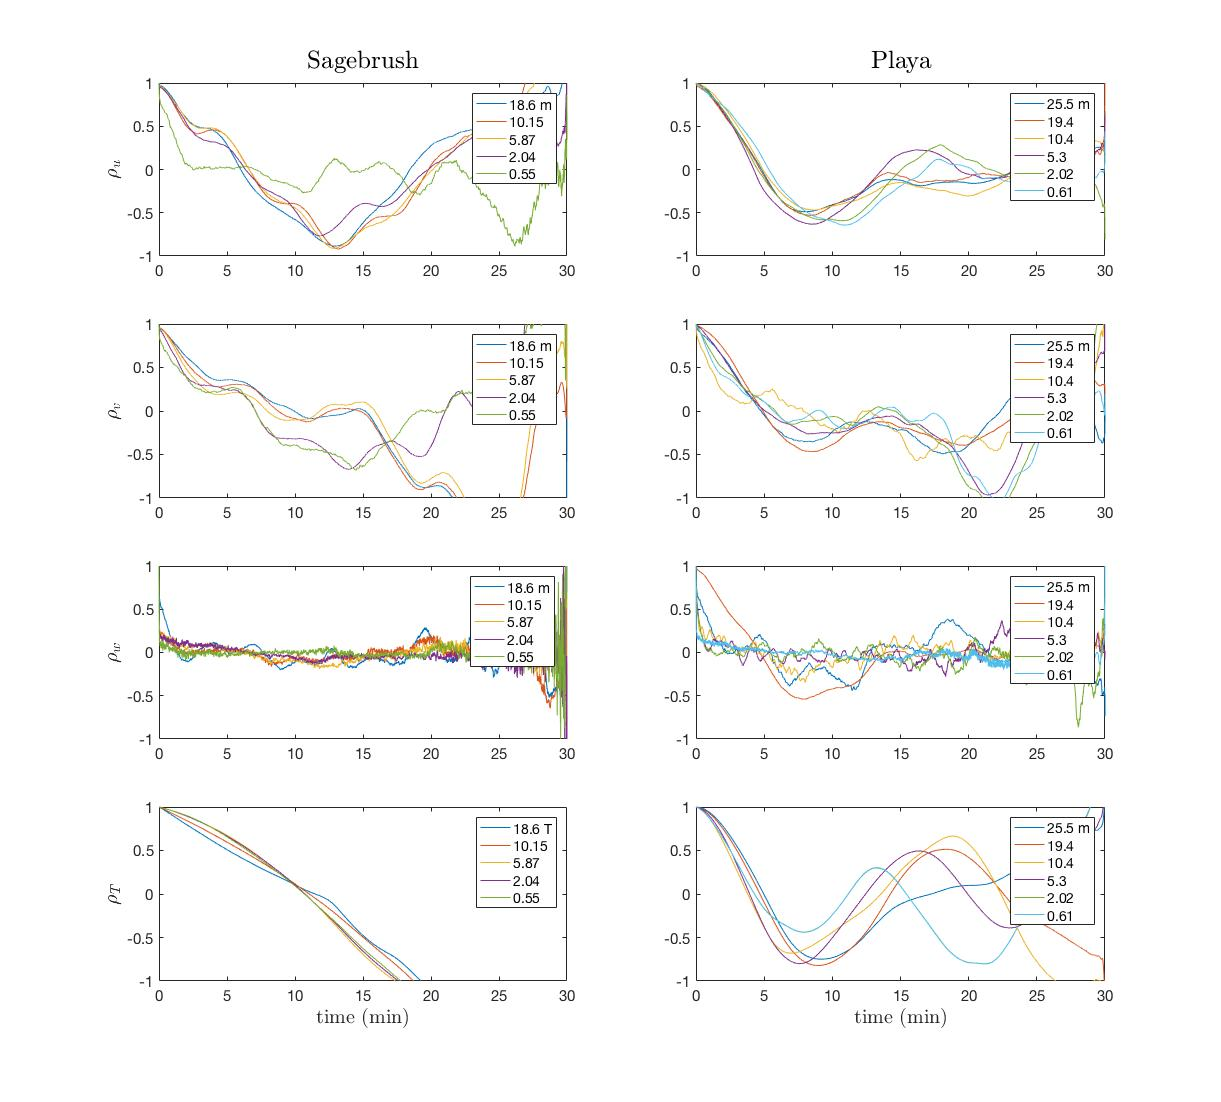
\includegraphics[width=\textwidth]{auto_corr_fig}
	\caption{}
	\label{fig:autocorr}
\end{figure}

%plot u mean, T mean u' v' and w'
\begin{figure}
	\centering
	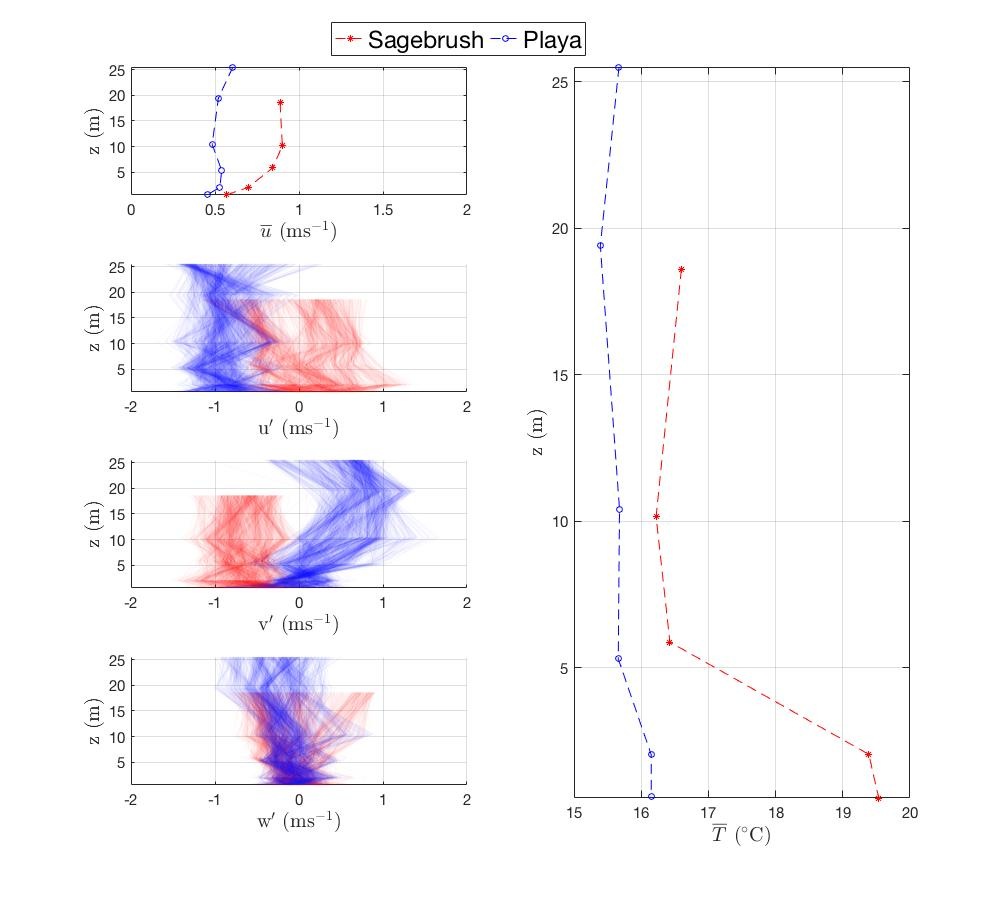
\includegraphics[width=\textwidth]{u_T}
	\caption{}
	\label{fig:u_T}
\end{figure}

\begin{figure}
	\centering
	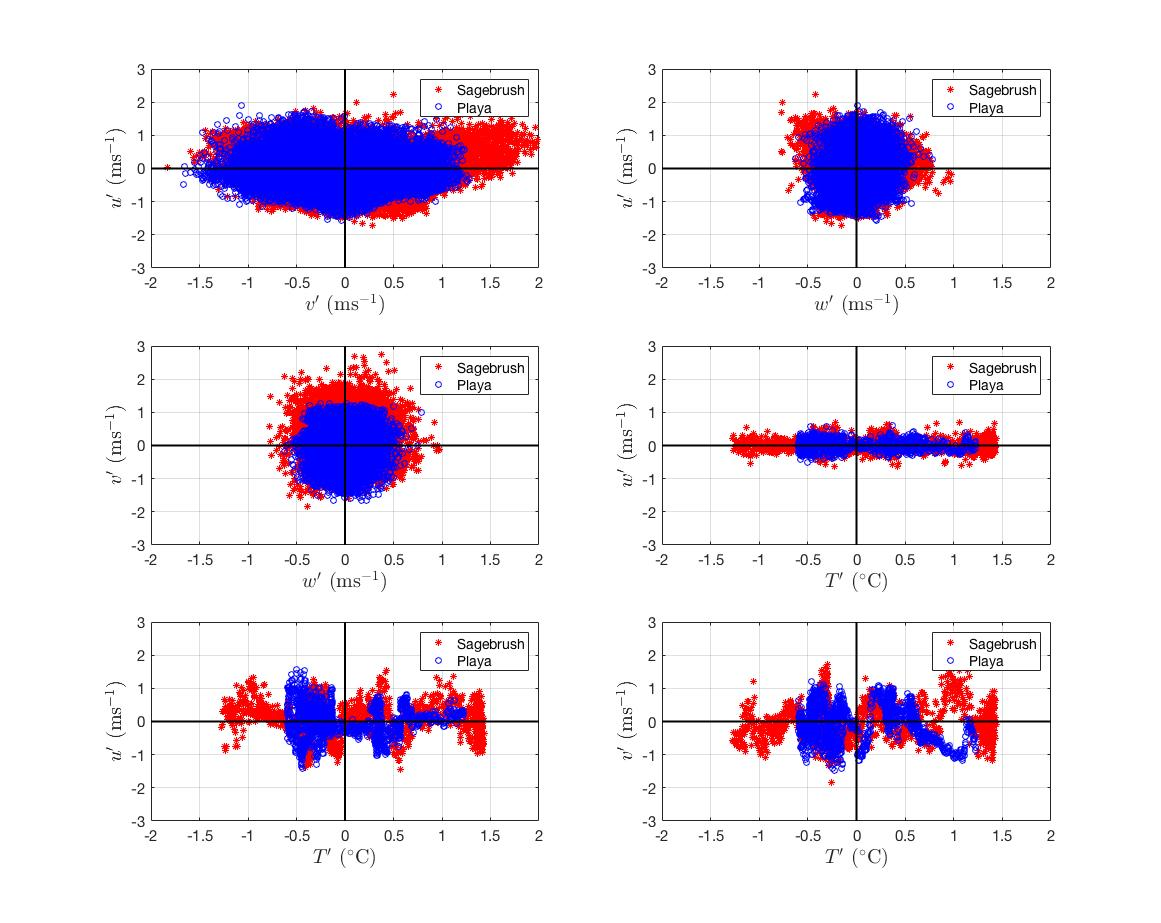
\includegraphics[width=\textwidth]{momentum_corr_05m}
	\caption{}
	\label{fig:u_T}
\end{figure}

\begin{figure}
	\centering
	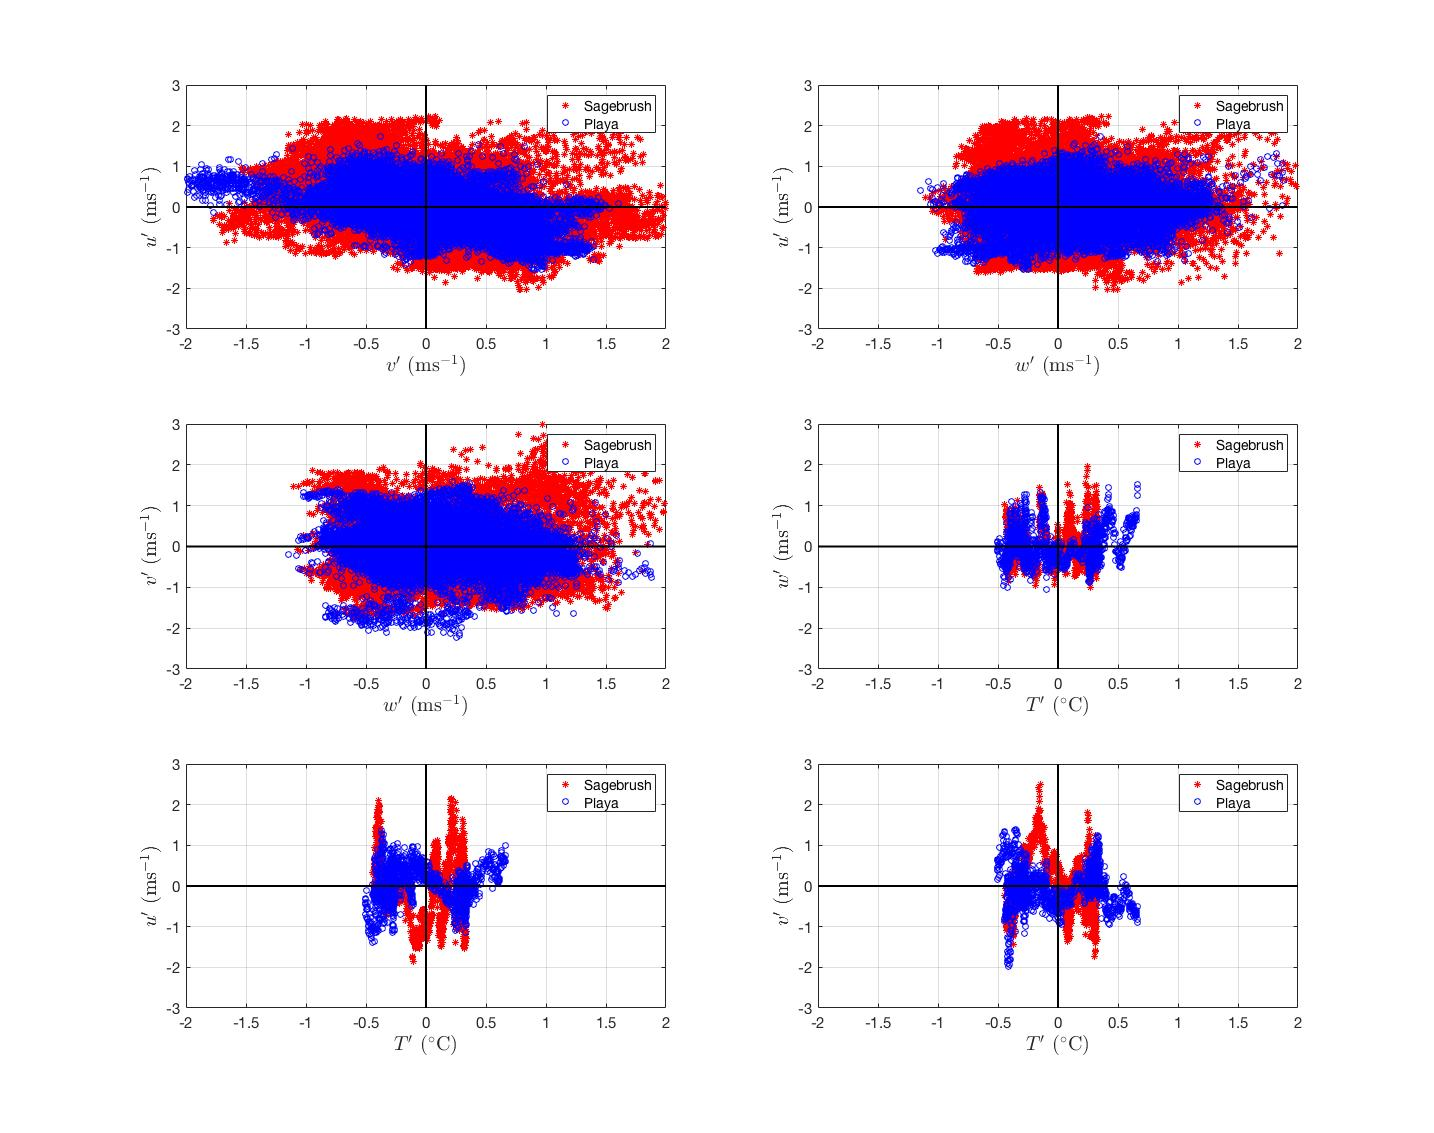
\includegraphics[width=\textwidth]{momentum_corr_20m}
	\caption{}
	\label{fig:u_T}
\end{figure}


%Matt talks about part 4 and 5

\section{Conclusion}


\end{document}
